\documentclass[../AISTR.tex]{subfiles}
\ifSubfilesClassLoaded{%
	\bibliography{../aistr}%
}{}
\begin{document}
\section{Составление документации по Modbus на Gitlab}
\subsection{Знакомство с языками разметки документации}
Документация на \textit{Gitlab} оформляется на языке разметки. \textbf{Язык разметки} -- набор символов или последовательностей символов, вставляемых в текст для передачи информации о его отображении или строении. 

Текстовый документ, написанный с использованием языка разметки, содержит не только сам текст (как последовательность слов и знаков препинания), но и дополнительную информацию о различных его участках:
\begin{itemize}
	\item заголовки;
	\item выделения;
	\item нумерованные и маркированные списки;
	\item таблицы.
\end{itemize}
Наличие языка разметки позволяет иметь документ одинакового вида на всех устройствах, что крайне важно для документации.
\subsubsection{HTML}
\textbf{HTML} -- стандартизированный язык разметки документов в сети Интернет. Большинство веб-страниц содержат описание разметки на языке HTML. Язык HTML интерпретируется браузерами; полученный в результате интерпретации форматированный текст отображается на экране монитора компьютера или мобильного устройства.

В листинге \rbf{list:html} приведён пример кода на языке HTML. На \refris{fig:html} приведён пример разметки, выполненной на языке HTML.

\begin{lstlisting}[caption=Пример кода на языке HTML,captionpos=b, label={list:html}]
	<html>
	<head>
	<meta http-equiv="Content-Type" content="text/html; charset=utf-8">
	<title>Пример веб - страницы</title>
	</head>
	<body>
	<h1>Заголовок</h1>
	<!-- Комментарий -->
	<p>Первый абзац.</p>
	<p>Второй абзац.</p>
	</body>
	</html>
\end{lstlisting}

\begin{figure}[h]
	\centering
	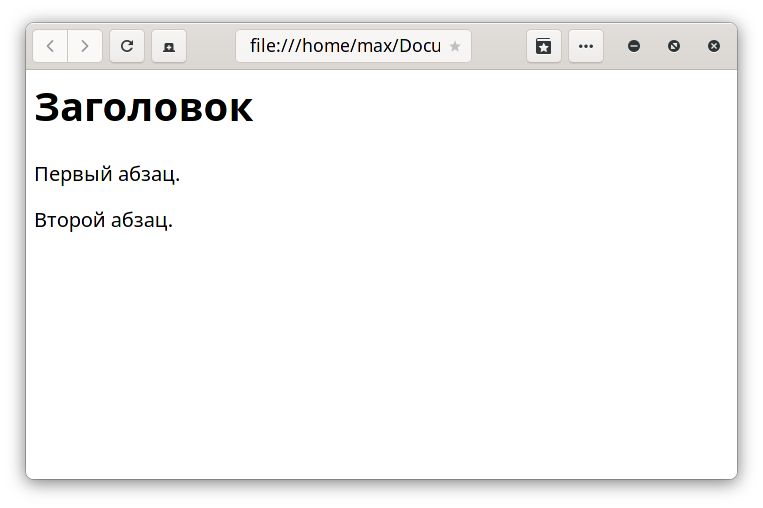
\includegraphics[trim=2 5 2 6,clip,width=0.7\linewidth]{../images/html}
	\caption{Результат выполнения примера}
	\label{fig:html}
\end{figure}
\subsubsection{Markdown}
\textbf{Markdown} -- облегчённый язык разметки, созданный с целью обозначения форматирования в простом тексте, с максимальным сохранением его читаемости человеком, и пригодный для машинного преобразования в языки для продвинутых публикаций (HTML, Rich Text и других).

Этот язык разметки намного проще \LaTeX и HTML, поэтому документация была перенесена на него.

На \refris{fig:md} приведён пример оформления документа на языке Markdown.
\begin{figure}
	\centering
	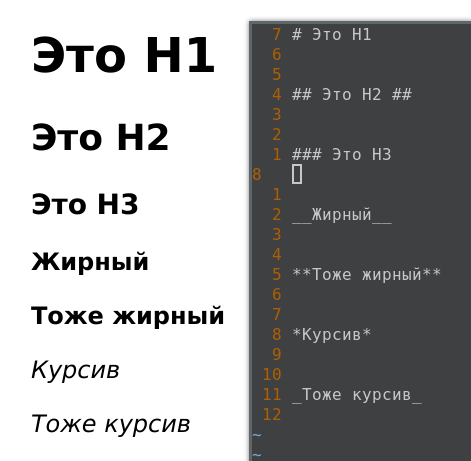
\includegraphics[width=0.5\linewidth]{../images/md}
	\caption{Пример кода на языке разметки Markdown}
	\label{fig:md}
\end{figure}

\subsection{Структурирование и перенос информации}
Информация со старого сервера была проработана и структурирована с использованием документации Modbus Foundation и наработок Л.Л. Колесника. На \refris{fig:result} показана часть переведённой с языка HTML на язык Markdown документации по протоколу \mb.

\begin{figure}
	\centering
	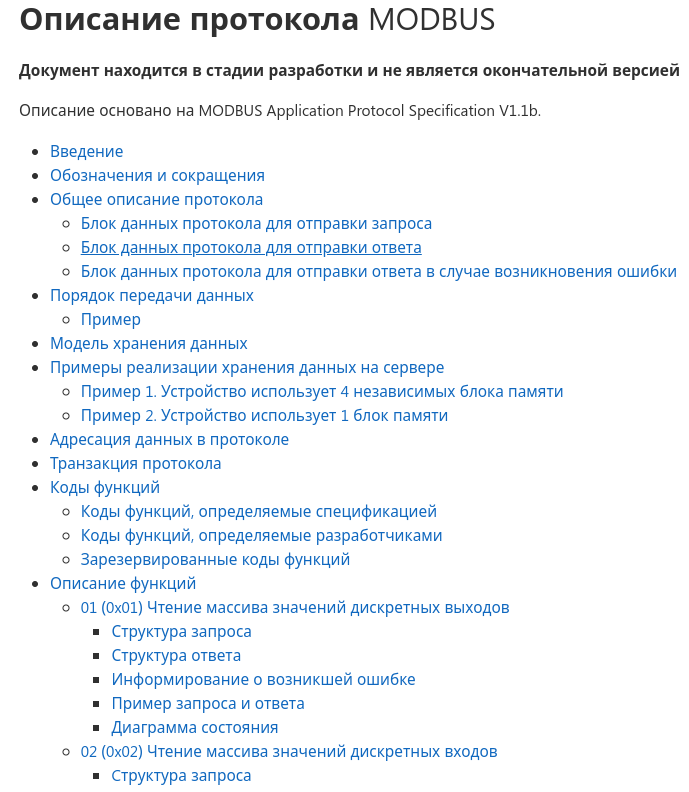
\includegraphics[width=0.9\linewidth]{../images/result}
	\caption{Информация в структурированном виде}
	\label{fig:result}
\end{figure}


\end{document}